\section{Adaptive Scheduling with Early Congestion Notification}
\label{sec:adaptive_with_ecn}

In this section, we propose modifications required for adaptive power scheduling algorithm~\cite{acsmartgrid} to support Early Congestion Notification (ECN) obtained from the ECN capable transport. We explain ECN mechanism in \ref{sec:explain_ecn} and then propose the integration of ECN in scheduling algorithm in \ref{sec:sched_ecn_integration}.

\subsection{Early Congestion Notification Mechanism}
\label{sec:explain_ecn} 

Congestion detection and avoidance for TCP through ECN (Early Congestion Notification) 
was proposed in~\cite{floyd1994tcp}. Essentially, ECN mechanism is implemented by 
maintaining two bits in IP header making four possible combinations as in 
Table~\ref{tab:ecn_bits}. If $ECT, CE$ are $0,0$ then the transport(Sender, Receiver, Network)
is considered to be not ECN-capable. If $ECT, CE$ are $0, 1$ or $1, 0$ then the transport is
ECN-capable and if $ECT, CE$ are $1, 1$ then the transport is ECN-capable but also the packet into
consideration has experienced congestion. 

{\bf Gateways,} in the network maintain $Q_{min}$ and $Q_{max}$ thresholds for average queue size $Q_{avg}$ for every
outgoing port. When a packet arrives at the gateway, one among the following actions is taken,

\null
IF $Q_{min} \geq Q_{avg} \leq Q_{max}:$ Set ECN bit. 

IF $Q_{avg} < Q_{min}:$ Take no action.

IF $Q_{avg} > Q_{max}:$ Drop packet.

\null
{\bf Receiver,} upon arrival of packet with ECN bit set (Congestion experienced), sets a flag in the acknowledgment 
packet header and send it back to Sender.

{\bf Sender,} when receives this acknowledgment (having congestion flag set), reduces the rate of transmission in order to avoid possible upcoming 
congestion. For example, in TCP, sender reduces the transmission rate by reducing its congestion window size and slow start threshold.
This mechanism avoids the unnecessary packet drops during mild congestion. As stated in~\cite{marekecnstudy}, ideally, marking based
network can avoid congestion through cooperative actions of responsive sources and completely eliminate packet drops.

	Although there are variations of ECN, such as Backward ECN (BECN)~\cite{Davidebecn, Davidebecnv2}, Forward ECN (FECN)~\cite{jiangfecn}, 
Enhanced Forward ECN (E-FECN)~\cite{jiangefecn}, we experiment using the congestion notification obtained from the receiver in acknowledgment 
packets (power acknowledgments in smart grid context).
	
\begin{table}
\begin{center}
\textit{RFC 3168}   
  \begin{tabular}{| l | c || r |}
   	\hline
   	ECT & CE & Codepoint \\ \hline
   	0 & 0 & Not-ECT \\
   	0 & 1 & ECT(1) \\
   	1 & 0 & ECT(0) \\
   	1 & 1 & CE \\
   	\hline
 \end{tabular}
    \caption{ECN Field In IP Header}
    \label{tab:ecn_bits}
\end{center}  
\end{table}	
		
\subsection{Integration: Scheduling With ECN}
\label{sec:sched_ecn_integration} 

	According to original scheduling algorithm, deadline miss event is triggered at a sender node $s$ when an acknowledgment $m_a$ of a message $m$ is not received before its deadline $d$. Reason for deadline miss is longer response time $RT$ (Round-Trip Time of $m$) than expected. $RT$ is affected by factors such as, link delays, increase in traffic (sharing same path in network) leading to queue buildup at gateways and processing delay at receiver. 

	In ECN capable transport, as stated in section~\ref{sec:explain_ecn}, if $Q_{avg}$ reaches $Q_{min}$, message $m$ is marked as congestion experienced (ECN bit is set in $m$). When sender $s$ detects ECN bit set in acknowledgment $m_a$, it is not guaranteed that $m_a$ will have a larger $RT$ than the system is currently expecting ($RT_s^{ex}$). ECN is just an indication of \textit{impending}  congestion. Thus, $m_a$ with ECN bit set may not trigger a deadline miss event, or will not cause the rate to reduce.	Therefore, to adapt due to ECN, we introduce a boolean flag $ECN_{Status}$ and a new sub event \textit{Detected ECN} under \textit{Ack Received Event} in the scheduling algorithm. Depending on $ECN_{Status}$ the scheduling algorithm changes its behavior dynamically and switches between the following modes,\\\\
{\bf Normal Mode: $ECN_{Status}(0)$: } No congestion detected. Algorithm runs as per section 4.1.\\\\
{\bf ECN Mode: $ECN_{Status}(1)$: } ECN mode is activated when a first acknowledgment is received indicating congestion. Figure. \ref{fig:ECN_flow} shows the flowchart of \textit{Ack Received} event in ECN capable transport. In this mode, $ECN_{Status}$ is set to $1$, $RTCtr$ is reset to zero and $RT_s^{ex}$ is incremented by $K_s*RTMargin$ instead of increasing by only $RTMargin$, as done in \textit{Deadline Miss} event. If $K_s < Kmax_s$, node parameters are recalculated using Equations \ref{rate-eq} - \ref{deadline-eq}. Otherwise, $r_s$ is set to $1/RT$ and other node parameters are calculated using Equations \ref{period-eq} and \ref{deadline-eq}. As we increase $RT_s^{ex}$ in proportion to $K_s$ (outstanding messages of sender node), rate $r_s$ of power transfer also reduces in proportion to $K_s$. ECN mode remains active for currently observed $RT$, after that it is deactivated and the algorithm returns back to Normal mode. The reason to do this is to avoid frequent adaptations due to acknowledgments indicating congestion. In a simple sense, ECN mode is activated only if the algorithm is currently running in Normal mode. Switch from ECN mode to Normal mode is implemented by $ECN\_Mode\_Dact\_t$ variable. \\


{\bf Problem. }Message acknowledgments received after the scheduling algorithm has switched to ECN mode, might have similar or even better (smaller) $RT$ to that of the first acknowledgment which caused the algorithm to switch to ECN mode (ECN being indication of \textit{impending} congestion). In this scenario, if $CtrMax$ number of consecutive acknowledgments are received with better $RT$, then adaptation due to better $RT$ will be performed, essentially, sub event \textit{Ack received is better} in \textit{Ack Received} will be triggered. In sub event \textit{Ack received is better}, message transfer rate $r_s$ is increased and tighter deadline $D_s$ is calculated. Thus, the efforts made to avoid congestion (by reducing $r_s$) after switching to ECN mode are compensated. The rate $r_s$ decreased after switching to ECN mode is again increased by triggering of \textit{Ack received is better}, because $CtrMax$ number of messages are most likely to appear consecutively with better $RT$. 


\begin{equation}
r_s = \frac{(Kmax_s - K_s)}{RT_s^{ex}} 
\label{rate-eq}
\end{equation}	

\begin{equation}
p_s = \frac{1}{r_s}
\label{period-eq}
\end{equation}

\begin{equation}
D_s = RT_s^{ex} + RTMargin
\label{deadline-eq}
\end{equation}

\begin{figure*}[htb]
  \begin{center}
%    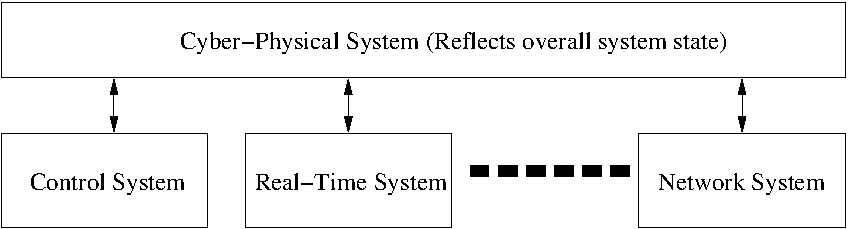
\includegraphics[width=0.45\textwidth]{Figures/cps-n-domains.pdf}
%    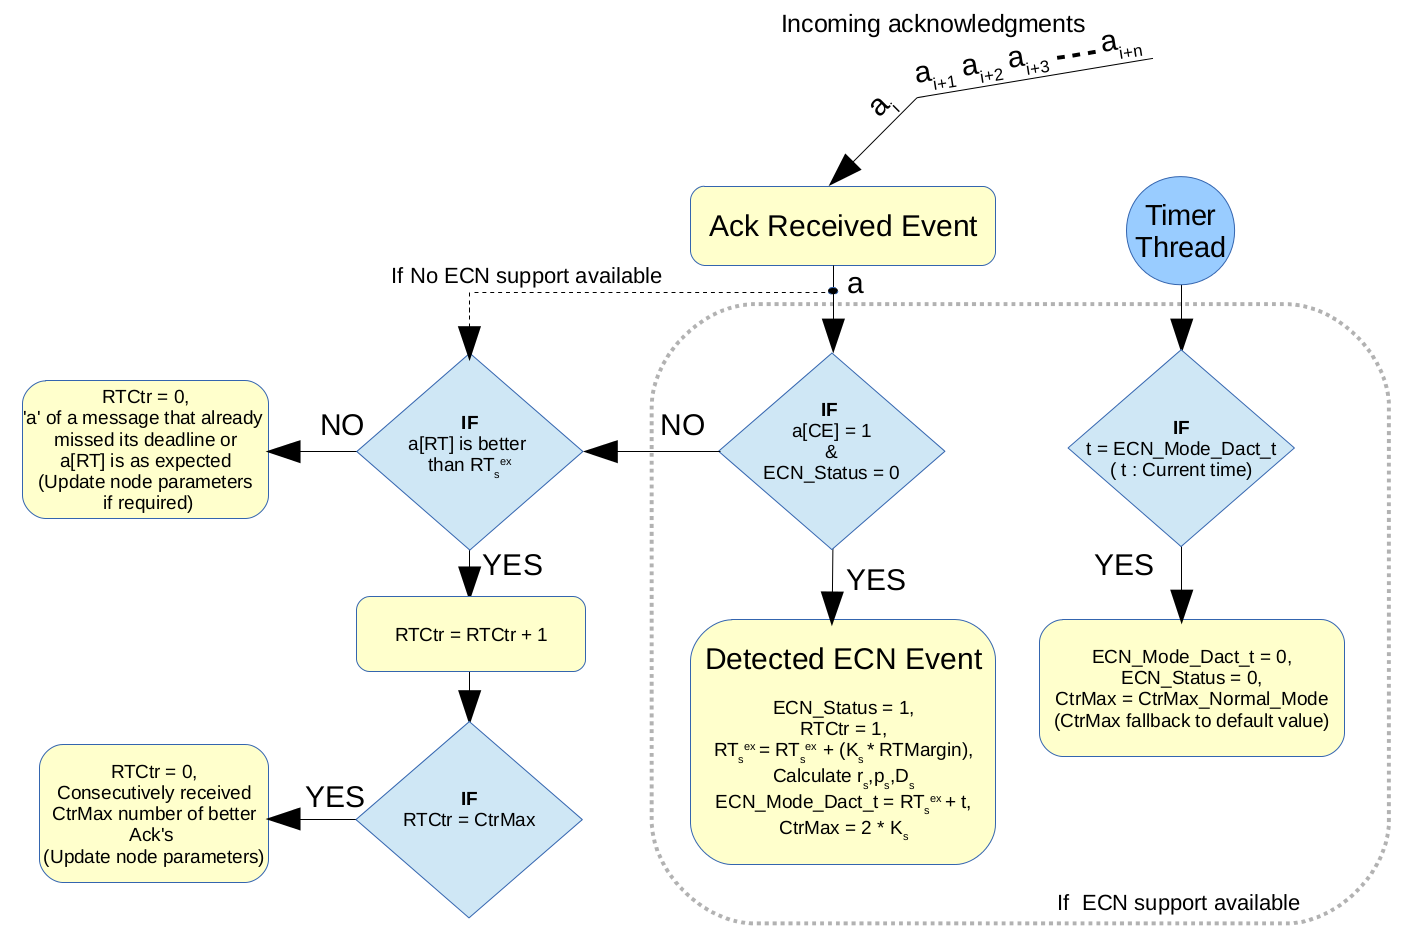
\includegraphics[width=0.9\columnwidth]{Figures/iccps2014/ECN_flow.png}
    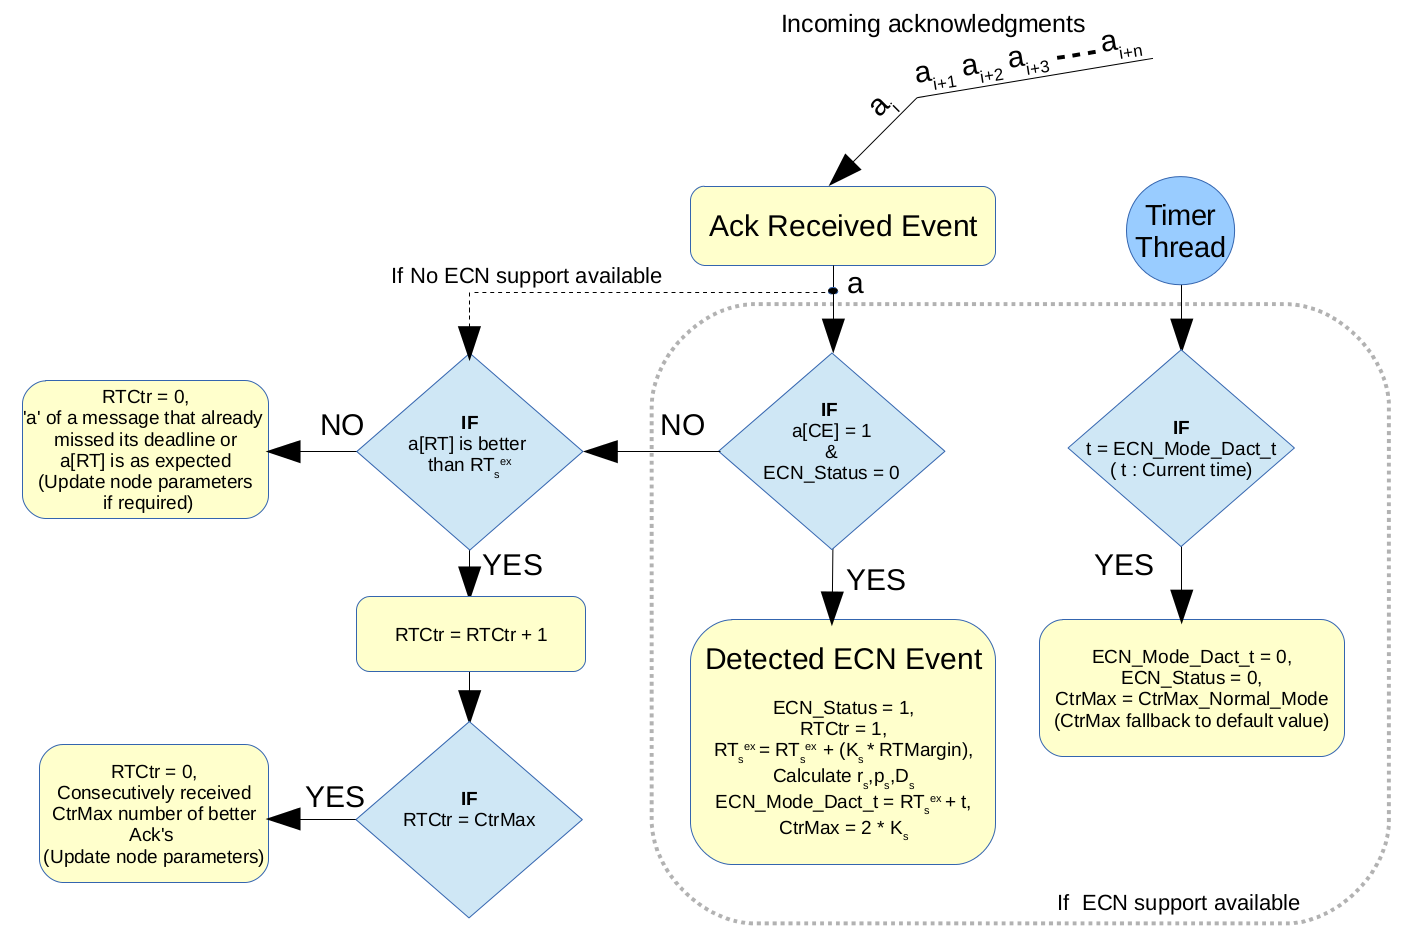
\includegraphics[scale=0.34]{Figures/iccps2014/ECN_flow.png}
  \caption{Flowchart Of $Ack ~Received$ Event With ECN Capable Transport}
  \label{fig:ECN_flow}
  \end{center}
\end{figure*}

{\bf Solution. }To avoid triggering of \textit{Ack received is better} event in ECN mode, we increase the $CtrMax$ limit to $2*K_s$, as shown in Figure.\ref{fig:ECN_flow}, in \textit{Detected ECN} event block. Increasing $CtrMax$ does not completely eliminate the triggering of \textit{Ack received is better} event, but instead makes it more tough to happen. Although $CtrMax$ is a configurable parameter in ECN mode, similar to as in Normal mode, we recommend setting the value of $CtrMax$ proportional to outstanding messages $K_s$. Note that $CtrMax$ is calculated only once per ECN mode switch.

\section{Varying Quantum Of Power ($\delta$)}
\label{sec:vary_delta} 

In previous section, we have successfully integrated a feature of ECN in our adaptive power message scheduling algorithm.
In this section we make changes to the policy of amount of $\delta$ carried by every power transfer message.
The idea is to vary $\delta$ size in proportion to period $p_s$ (or 1/rate, $1/r_s$). But when we talk about 
internet like network, it is non-trivial to bound the rate of transmission. So, each time a message scheduling 
invariant $I_S$ is evaluated, we make an estimate on total amount of power that can be transferred in the  
current power transfer phase $PT$, provided, the current scheduling parameter $r_s$ (rate) does not change.
Based on this estimate, we calculate $\delta$ as in Equation.\ref{eqn:delta_calc}. 

\begin{equation}
\delta = \frac{P_G - P_A}{r_s * (PT_e - RT_s^{ex})} 
\label{eqn:delta_calc}
\end{equation}	

Where, $P_G$ is total power granted to receiver node $r$, $P_A$ is total power acknowledged from node $r$
(node $r$ (receiver node's) stamps total power received in current $PT$ (power transfer phase) in every $ack$), $r_s$ is current rate of power transfer message,
$PT_e$ is absolute end time of current power transfer phase and $RT_s^{ex}$ is current observed response time of
message.

{\bf Problem. }Message scheduling invariant $I_S$ formed by conjunction of sub invariants $I_k$, $I_c$ and $I_p$, will not reflect 
the correct scheduling system state if $\delta$ is allowed to vary. As $I_k$, satisfied if $K_s$<$K_{max_s}$, no more reflects 
the amount of outstanding power in the grid. $K_s$ only reflects the total outstanding messages in the network, because in varying 
$\delta$ scenario, every power transfer message might carry different amount of $\delta$ along them. 

{\bf Solution. }We derive the bounds on $\delta$ as, $\delta_{min}$ and $\delta_{max}$ based on the physical system tolerance
(allowance) [****input from physical system guys that $\delta_{min}$ and $\delta_{max}$ can be provided, ensuring that the 
system stability won't be affected] without compensating for stability. Now in the physical system analysis, in section\ref{sec:invariants},
where we say "$I_{P1}$ ultimately imposes a limit on $\delta * K$", will not hold. Therefore, we modify the term $\delta K$ 
in Equation 3 to $P_T - P_A$ and restate the Equation as in \ref{eqn:grid4_modified}. 

\begin{equation}
\left\{
\begin{matrix}
I_{P1}: (\omega - \omega_0)^2 \left(D\omega + m \right) \\ + (\omega - \omega_0)(kP^2)  > (P_T - P_A)(\omega - \omega_0)
\end{matrix}
\right\}
\label{eqn:grid4_modified}
\end{equation}

Where, $P_T$ is the total power transferred to node $r$ (receiver node) and 
$P_A$ is the total power acknowledged from node $r$. (Note that $P_G$ is total 
power granted, power transfer stops due to the end of $PT$ or $P_G$ = $P_T$ = $P_A$).

We also modify the sub invariant $I_k$ in scheduling invariant $I_S$ as in
Equations \ref{eqn:mod_Ik}-\ref{eqn:mod_Ikn}.

%\begin{equation}
%I_k: I_{kp} \wedge I_{kn} \wedge I_{kd}
%\label{eqn:mod_Ik}
%\end{equation}	

\begin{equation}
I_k: I_{kp} \wedge I_{kn}
\label{eqn:mod_Ik}
\end{equation}	

\begin{equation}
I_{kp}: (\delta_{new} + (P_T - P_A)) < (\delta_{max}*K_{max_s})
\label{eqn:mod_Ikp}
\end{equation}	

\begin{equation}
I_{kn}: K_s < K_{max_s}
\label{eqn:mod_Ikn}
\end{equation}	

%\begin{equation}
%I_{kd}: (\delta_{new} + (P_T - P_A)) < (\delta_{max}*K_{max_s})
%\label{eqn:mod_Ikd}
%\end{equation}	

Where, $\delta_{new}$ is obtained from Equation ~\ref{eqn:delta_calc}.






